\chapter{Online and Distributed Boosted Trees}

In this chapter we provide an overview of our work on developing a distributed
algorithm for online boosting. We provide an introduction to the problem
in Section \ref{sec:boostvht-background}, describe the methods we developed
in Section \ref{sec:boostvht-method}, and present our experimental results
in Section \ref{sec:boostvht-results}.

\section{Background}
\label{sec:boostvht-background}

% Describe the problem
Boosting algorithms are some of the most successful and widely used algorithms
in machine learning, due to their simplicity and excellent accuracy. As a result,
a wide array of research has been proposed with the aim of improving the scalability
of boosting, either through parallelizing the base algorithm, or by developing
algorithms that can perform boosting online.

% Previous approaches and why they don't work
However, there exists a disconnect
between these different paths to scalability: Most parallel boosting algorithms
only work in a data-parallel setting, that is, by training multiple examples simultaneously.
They maintain a weight distribution for the complete dataset, and, after iterating through the complete dataset, they adjust each example's weight
and continue learning.
On the other hand, online boosting algorithms work by passing each example through
the boosting chain, updating each learner in sequence, and the weight of the instance
as it passes through each learner.
This presents a problem in creating a parallel \textit{and} online learner: The
existing parallel boosting literature require that the complete dataset is available
to maintain a weight distribution over the data, while online boosting algorithms
use a strictly sequential process for each data point, eliminating data-parallelism.

% Our method
In this work we aim specifically at this gap in current research: \emph{online and parallel
boosting}. In order to provide parallelism while maintaining the guarantees of existing
online boosting algorithms, we use a sequential ensemble of model-parallel learners that train
on different parts of a single data point in a distributed environment.

\section{Method}
\label{sec:boostvht-method}

Our method makes use of the Vertical Hoeffding Tree (VHT) algorithm \cite{kourtellis2016vht} which is a model-parallel
extension of the online Hoeffding tree algorithm \cite{vfdt}, often referred to as
Very Fast Decision Tree (VFDT)\todo{Make sure we have talked about the VFDT in the background}.
The VFDT algorithmn will sort instances down the tree and update the statistics for the
leaf the instance ends up in. This separation of duties allows for the scalable design of
VHT: the algorithm uses two components, one called the \emph{model aggregator}
that is responsible for sorting instances to leafs and maintaining the model, and
one called the \emph{local statistics}, which are potentially many workers responsible
for maintain the statistics for the leaves of the tree.
The model aggregator is responsible for breaking up each instance into its constituent
features, and sending them, along with the label, to the local statistics workers.
The model aggregator will periodically query the local statistics to check if we have
collected enough information to split the leaf with high confidence, as done in the
original VFDT.

Our method makes use of the VHT in order to enable parallelism in online boosting,
and proposes optimizations that make the learning process efficient in a distributed
setting. We use a design that is similar to the original VHT in that we maintain
two main components, one model aggregator and local statistics. However, our model
aggregator hosts a sequential chain of VHT models, though which we pass each example.
This design allows us to maintain the sequential nature of the boosting algorithm,
and as a result the guarantees of any online boosting algorithm, while performing
the training in parallel and asynchronously in a set of local statistics workers.

We propose three optimizations over the original VHT algorithm to improve its
characteristics for distributed boosting. First, we design our local statistics
so that the same worker can host statistics from multiple member of the ensemble.
This enables to decouple the level of parallelism from the number of learners
in the ensemble, separating the algorithm's functional (speedup) and non-functional
(accuracy) constraints.
Second, this enables us to host the statistics for a range of features on the same
worker, across all the ensemble. This makes our communication pattern efficient:
We only need to send $p$  messages per instance, where $p$ is the chosen
parallelism level, compared to sending $m$ messages, where $m$ the
number of features. This will dramatically
reduce the number of messages sent, since we expect $m \gg p$. In addition, compared to existing
parallel boosting methods like AdaBoost.PL \cite{adaboost-pl} that need to communicate the complete
models between update, we only need to communicate the split decisions which are
much more compact.
Finally, our approach allows us to send each attribute slice only once to
each worker, as it suffices for each subsequent learner after the first
to only send their updated weight. This brings a communication reduction
of a factor $s$, where $s$ is the ensemble size, which can often be hundreds of
trees~\cite{hundreds-classifiers}.

\section{Main Findings}
\label{sec:boostvht-results}

For our experiments we use 10 artificial and 4 real-world datasets. The artificial
datasets are generated with different numbers of attributes using one generator
from a tree-like structure, one that generates random tweet text for a sentiment
analysis task, and one rotating hyperplane. The baselines we test against are
a single-threaded online boosting algorithm from the MOA \cite{bifet2010moa}
library using the Hoeffding tree as a base learner, and the base VHT tree.
We measure the speedup over the single-threaded algorithm, and use the
robust Kappa\cite{bifet2015efficient} statistic to measure accuracy,
that considers the probability of agreement by chance in the evaluation.

We start by showing that the boosted version of the algorithm performs
better than the base VHT. Figure \ref{fig:boostvht-textgen-accuracy} shows an example experiment using different
levels of dimensionality for the text-generator data. We can see
that as we increase the number of features and make the problem more
difficult, the accuracy of the VHT algorithm deteriorates, while
BoostVHT is consistently accurate, and is able to match the performance of the single-threaded
boosting algorithm.

\begin{figure*}
	\centering
	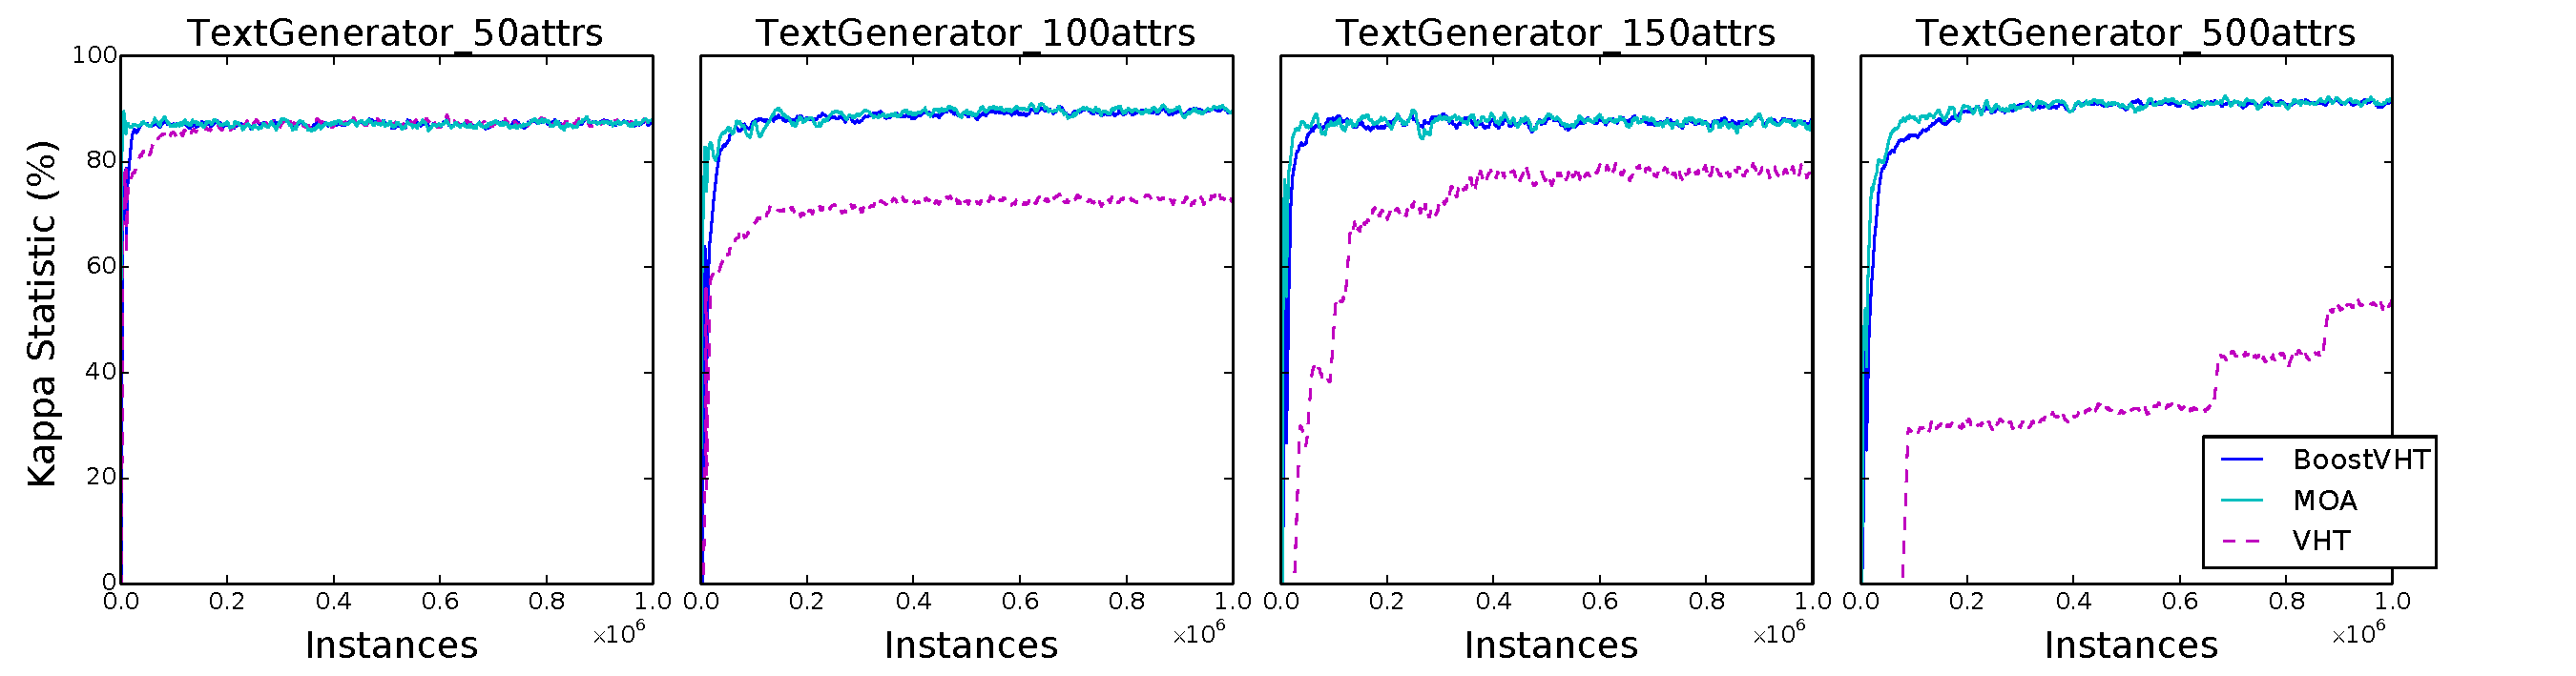
\includegraphics[width=\textwidth]{textGen_all_kappa_stat_storm.pdf}
	\caption{Kappa statistic (accuracy) as a function of arriving instances over time for text generator datasets with
		an increasing number of attributes.}
	\label{fig:boostvht-textgen-accuracy}
\end{figure*}

In the paper we further demonstrate that BoostVHT is able to maintain an accuracy almost equivalent to
the single-threaded boosting algorithm, while providing a speedup of 45x on average.
Finally we examine the scalability of the algorithm in terms of strong and weak scaling.
Ideal strong scaling provides \emph{linear speed-up}: Doubling the amount of resources
while keeping the problem size constant should halve the execution time.
Ideal weak scaling should have \emph{linear scale-out}: doubling both the problem size
and resources at the same time should affect the training time significantly.
We illustrate the scaling characteristics of the algorithm in Figures
\ref{fig:weak-scaling} and \ref{fig:strong-scaling} for weak and strong
scaling respectively. As we can see in the figures, the algorithm scales
almost ideally both in terms of weak scaling, keeping its training time
close to constant as we double resources and the problem size, and provides
near-linear speed-up for our strong scaling experiments.

\begin{figure}
	\centering
	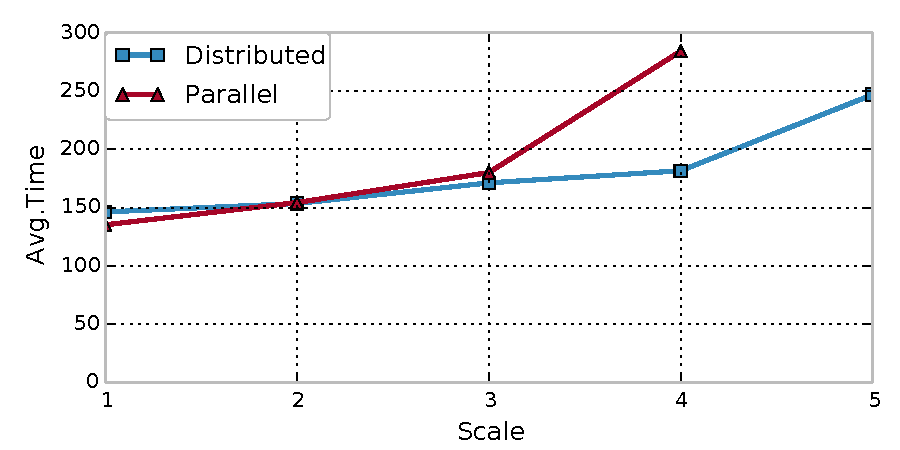
\includegraphics[width=0.8\textwidth]{weak-scaling.pdf}
	\caption{Weak scaling experiments, time in milliseconds. Scale 1x on the x-axis refers to 500 attributes with 2 Processors, and we double both Processors and attributes for each scale increment (up to 8,000 attributes with 32 Processors).}
	\label{fig:weak-scaling}
\end{figure}

\begin{figure}
	\centering
	\begin{subfigure}[t]{0.5\textwidth}
		\centering
		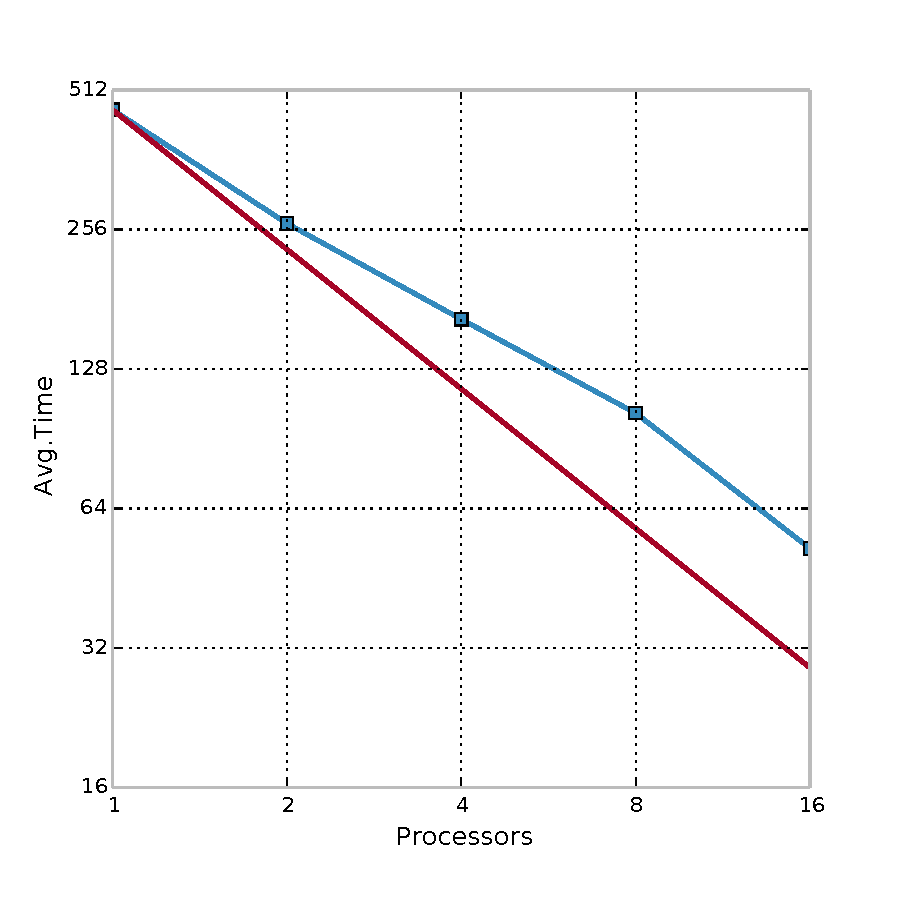
\includegraphics[width=\linewidth]{ice-strong-scaling.pdf}
		\caption{Parallel experiments.}
		\label{fig:strong-parallel}
	\end{subfigure}%
	\begin{subfigure}[t]{0.5\textwidth}
		\centering
		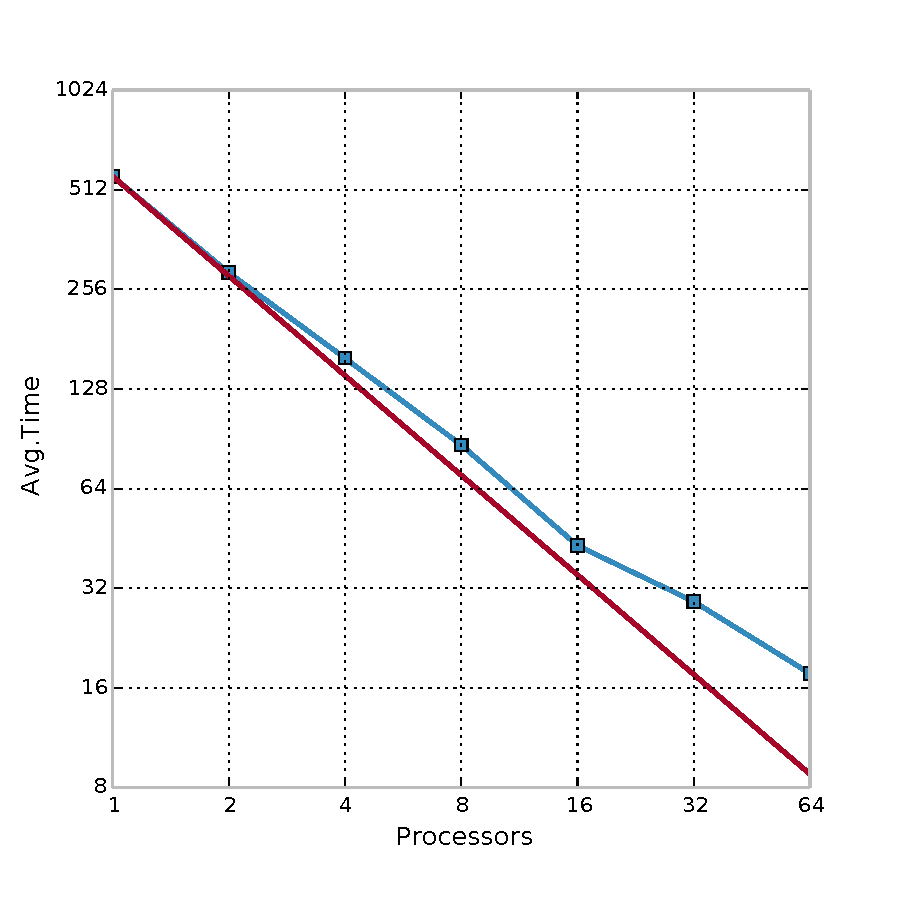
\includegraphics[width=\linewidth]{ec2-strong-scaling.pdf}
		\caption{Distributed experiments}
		\label{fig:strong-distributed}
	\end{subfigure}
	\caption{Strong scaling in the parallel (left) and distributed (right) setting. The
		time reported is the average time to train 1,000 instances, each with 1,000 attributes, in milliseconds. The red straight line indicates ideal linear scaling.}
	\label{fig:strong-scaling}
\end{figure}